\documentclass[11pt,a4paper]{report} 

\usepackage[utf8]{inputenc} 
\usepackage[norsk]{babel} 
\usepackage{lipsum,paralist}
\usepackage{graphicx}
\usepackage{array}
\usepackage{longtable}
\graphicspath{ {./images/} }


\begin{document}
\title{
Forprosjektrapport \\
\vspace{2cm}
Aktiv student \\
En digital plattform for synliggjøring og kontakt med frivillige organisasjoner \\
Gruppe nr 6
}
\author{
\LARGE
Stefan Larsen, Ingrid Elise Dahl  \\
\LARGE
Markus Arnø Madsen, Anders Walle Pettersen \\
}
\maketitle

\section*{Prosjektgruppen}

Prosjektgruppen er sammensatt av tre studenter fra Digitale Medier og Design og én student fra Informatikk - Design og utvikling av IT-systemer.

Ingrid Elise Dahl studerer Informatikk - Design og utvikling av IT-systemer, bor i Halden og er fra Trondheim. Ingrids faglige interesser innebærer frontend-utvikling, design, datasikkerhet, databasesystemer og applikasjonsutvikling.

Markus Arnø Madsen studerer Digitale medier og Design, bor i Fredrikstad og er fra Trondheim. Markus sin faglige interesse innebærer design, prosjektledelse, interaksjons design, brukerorientert design, markedsføring og prosjekt/produkt utvikling.

Anders Walle Pettersen studerer Digitale medier og Design, bor i Fredrikstad. Anders sin faglige interesse innebærer design, interaksjons design, spillutvikling, grafisk design og brukerorientert design.

Stefan Larsen studerer Digitale medier og Design, og bor i Halden. 3D og Grafisk design, samt Webutvikling har vært noen av de mest interessante veiene å utforske gjennom studietiden på HIOF. 


\section*{Oppdragsgiver}

Gruppens oppdragsgiver er Tommy Payne ved Høgskolen i Østfold. Tommy jobber som Seniorkonsulent i Studieenheten ved Høgskolen i Østfold og inngår i team for Studieutredning og kvalitetssikring med ansvar for det helhetlige læringsmiljøet ved campus Halden og campus Fredrikstad. Arbeidet hans går ut på å sikre og videreutvikle det digitale, fysiske, organisatoriske og psykososiale læringsmiljøet ved høgskolen. [1]

\section*{Oppdraget}

Det kommer fram av Studentenes Helse -og Trivselsundersøkelse 2018 at nesten hver tredje student opplever ensomhet i studietiden. [2] Ved å bruke Frivillighetsregisteret på Brønnøysundsregisteret sine nettsider har gruppen som oppdrag å lage en nettbasert plattform som gjør det enklere for studenter å finne frivillige organisasjoner, lag og foreninger i sitt nærområde.

Oppdragsgiver Tommy Payne jobber blant annet med læringsmiljø og studentenes trivsel og helse ved Høgskolen i Østfold. Å utvikle en plattform som hjelper studenter å bli mer aktive, delta mer sosialt og engasjere seg i lokalmiljøet vil være av interesse for både Tommy Payne, Høgskolen i Østfold og nærmiljøet rundt Høgskolen.

Plattformen skal utvikles som et Wordpress-nettsted. Informasjon skal hentes ut fra Frivillighetsregisteret, oppdateres jevnlig og vises i et hensiktsmessig format. Brukere skal kunne filtrere søk etter interesse og område og enkelt ta kontakt med organisasjoner.

\subsection*{Kravspesifikasjon}
Det fins en rekke primærkrav som er definert av oppdragsgiver. Gruppen har i tillegg valgt å definere sekundær som ikke \em må \em være med i produktet men som \em kan \em eller \em bør \em være med om det blir nok tid og ressurser til dette.

\subsubsection{Primærkrav: hva \em må \em være med i produktet}
\begin{itemize}
\item Kunne søke opp eksisterende lag, foreninger og organisasjoner i nærområdet rundt Høgskolen i Østfold
\item Vise navn, kategori, geografisk sted, eventuell nettside og kontaktinformasjon for organisasjonene
\item Benytte fritekstsøk ut fra organisasjonsnavn i kombinasjon av valgte filter og søkekriterier
\item Skal kunne brukes av studenter ved Høgskolen i Østfold
\item Nettstedet skal være utviklet i Wordpress
\item Skal være enkelt å vedlikeholde av oppdragsgiver
\item Skal kunne takle små eventuelle endringer i datakilde
\item Skal kunne oppdatere infomasjon fra datakilden hver gang man oppdaterer nettsiden
\end{itemize}


\subsubsection{Sekundærkrav: hva \em kan \em være med i produktet}
\begin{itemize}
\item Kunne søke opp eksisterende lag, foreninger og organisasjoner i hele Norge
\item Kunne komme i kontakt med andre personer med samme interesse for å starte opp en ny organisasjon, lag eller forening
\item Kunne bruke systemet ved flere utdanningsinstitusjoner i Norge
\item Vise søkeresultater i interaktivt kart
\item Vise veibeskrivelse i kart til valgt resultat
\end{itemize}


\subsection*{Formål}

\begin{compactitem}
\item [{\bf Hovedmål}] Skape en løsning for studenter slik at de enklere kan få oversikt over og komme i kontakt med frivillige organiasjoner, lag og foreninger i sitt nærområde. Samt skape en bedre og enklere løsning en den som finnes idag. Dette vil igjen berike nærmiljøet og føre til mindre ensomhet blant studenter.
\begin{compactitem}
\item [{\bf  Delmål 1} ] Redegjøre for den gjennomsnittlige brukerens behov samt utrede hvilke ulike tekniske implementasjoner som er realistisk å kunne gjennomføre i utviklingsperioden.\\Frist: 27.02.2020
\item [{\bf  Delmål 2} ] Ha en kartlagt plan over hvordan den endelige produksjonen av nettstedet skal foregå.\\Frist: 29.02.20
\item [{\bf  Delmål 3} ] Ferdigstille versjon 1 av nettsted.\\Frist: 15.04.20
\item [{\bf  Delmål 4} ] Ferdigstille prosjekt til intern frist. Designet for å gi produksjonsteamet en bufferperiode på 3 uker før endelig leveranse av produkt. \\Frist 24.04.20
\end{compactitem} 
\end{compactitem}

\subsection*{Leveranser}

Det skal leveres et CMS bygd i Wordpress som bruker Frivillighetsregisteret som datakilde. Det leveres også teknisk dokumentasjon for at oppdragsgiver enkelt skal kunne overta og vedlikeholde produktet.

Hoveddokumentet, i tillegg til første og andre utkast av dette skal leveres. Forprosjektrapporten er også en del av leveransen. Det skal også leveres en hjemmeside med kort beskrivelse av prosjektet og link til leveranser. Mot slutten av prosjektperioden skal det leveres en prosjektplakat og individuelle refleksjonsnotater fra gruppemedlemmene.

\subsection*{Metode}
Relevante brukerundersøkelser av studenter. For å lage og fullføre vårt produkt på best mulig måte skal det brukes kunnskap og erfaring som har blitt anskaffet i studiene til prosjektgruppen. Det skal blant annet brukes mye fra prosjektledelse i selve forarbeidet for å planlegge utviklingen, samt implementeres faginnhold fra både brukerorientert design og designmetoder for å komme til den best mulige løsningen for utviklere kontra brukerene. Ved valg av utseende på nettstedet skal det brukes fagstoff og erfaring fra grafisk design og kommunikasjonsdesign til dette, og strukturen på siden skal bestå av faglige retningslinjer fra utvikling av interaktive nettsteder og informasjons arkitektur.


\section*{Prosjektplan}

\begin{compactdesc}
\item [Aktivitetet 1:] Forprosjektrapport
	\begin{compactitem}
	\item Start: 09.01.2020
	\item Slutt: 20.01.2020
	\item Bemanning: Alle
	\item Leveranse: Leveres som PDF til veileder, oppdragsgiver og fagansvarlig
	\item Beskrivelse: En overordnet beskrivelse av gruppen, oppdragsgiver, prosjektet og gjennomføring.
	\end{compactitem}
	\item [Aktivitetet 2:] Oversiktsplan
	\begin{compactitem}
	\item Start: 20.01.2020
	\item Slutt: 27.01.2020
	\item Bemanning Alle
	\item Leveranse: Denne planen blir presentert for både oppdragsgiver og veileder i et møte med hver av dem.
	\item Beskrivelse: En enighet mellom gruppen, veileder og oppdragsgiver om hvordan vi skal løse oppgaven og hvordan planleggingen og gjennomføringen av produktet skal utvikles. Dette blir presantert og diskutert med oppdragsgiver i et møte 28.01.2020
	\end{compactitem} 
	\item [Aktivitetet 3:] Brukerundersøkelse
	\begin{compactitem}
	\item Start: 14.01.2020
	\item Slutt: 27.02.2020
	\item Bemanning: Stefan, Anders
	\item Leveranse: Resultater fremlegges i møtet med oppdragsgiver 28.01.2020
	\item Beskrivelse: Formålet med brukerundersøkelsen er å forstå behovet til våre brukere, samt skape et overordnet forhold til navigasjon og informasjons arkitektur. 
	\end{compactitem}
	\item [Aktivitetet 4:] Fysisk plan for produktet
	\begin{compactitem}
	\item Start: 29.01.2020
	\item Slutt: 29.02.2020
	\item Bemanning Alle
	\item Leveranse: Planen vil bli presantert og godkjent av både veileder og oppdragsgiver. 
	\item Beskrivelse: En komplett plan med oversikt over hvordan og når de forskjellige delene av produktet skal konstrueres og forbredende faglig stoff og elementer som trengs for å lage produktet. Her skal kunnskap og erfaring fra våre grader og interesser brukes.
	\end{compactitem}
	\item [Aktivitetet 5:] Utvikling av produkt
	\begin{compactitem}
	\item Start: 30.02.2020
	\item Slutt: 15.04.2020
	\item Bemanning Alle
	\item Leveranse: Fremlegges i samråd med veileder for oppdragsgiver 
	\item Beskrivelse: Produktet utvikles under kontinuerlig burker testing.
	\end{compactitem}
	\item [Aktivitetet 6:] versjon 1 av hoveddokumentet
	\begin{compactitem}
	\item Start: 01.02.2020
	\item Slutt: 15.03.2020
	\item Bemanning Alle
	\item Leveranse: Fremvise progresjon kontinuerlig for veileder på veilednings møtene. 
	\item Beskrivelse: forprosjekt raport og dokumentasjon, i tillegg til vår progresjon hitil i prosjektet. 
	\end{compactitem}
	\item [Aktivitetet 7:] Brukertesting
	\begin{compactitem}
	\item Start: 15.03.2020
	\item Slutt: 22.04.2020
	\item Bemanning Alle
	\item Leveranse: Fremlegge testresultater for oppdragsgiver og løsningsplan ved eventuelle feil eller koregering. 
	\item Beskrivelse: Testing av det ferdige produktet.
	\end{compactitem}
	\item [Aktivitetet 8:] versjon 2 av hoveddokumentet
	\begin{compactitem}
	\item Start: 15.03.2020
	\item Slutt: 24.04.2020
	\item Bemanning Alle
	\item Leveranse: Fremvise progresjon kontinuerlig for veileder på veilednings møtene. 
	\item Beskrivelse: dokumentet skal være tilfredsstillende nok for en ståkarakter.
	\end{compactitem}
	\item [Aktivitetet 9:] finpuss og ferdigstilling
	\begin{compactitem}
	\item Start: 24.04.2020
	\item Slutt: 15.05.2020
	\item Bemanning Alle
	\item Leveranse: fremvise progresjon for veileder ved ukentlige møter. 
	\item Beskrivelse:ferdigstille hoveddokument.
	\end{compactitem}

\end{compactdesc}

\section*{Gjennomføring}

\subsection*{Risikoanalyse}

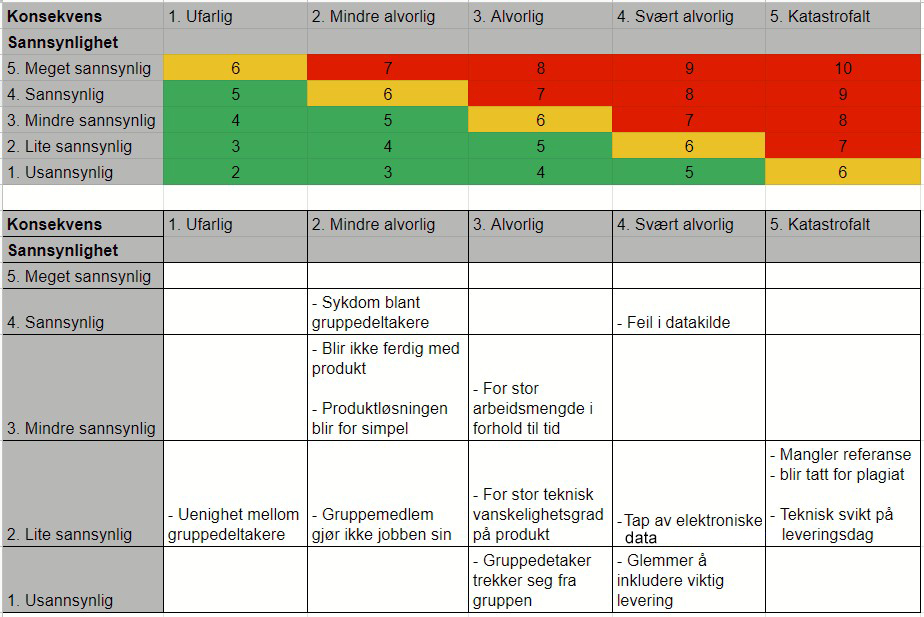
\includegraphics[scale=0.75]{ros-analyse}

\subsubsection*{Tiltak}
\begin{center}
\begin{longtable}{ |m{6cm}|m{7cm}| } 
 \hline
 \bf Problem \bf & \bf Tiltak \bf \\
 \hline
 Uenighet mellom gruppedeltakere & God kommunikasjon, variasjon mellom å jobbe hjemmefra og møtes. Snakke med emneansvarlig hvis konflikt ikke løses innad i gruppa. \\ 
 \hline
 Sykdom blant gruppedeltakere & Gruppemedlem jobber hjemmefra hvis den kan. Hvis ikke må de andre medlemmene ta personens oppgaver til den er frisk. \\ 
 \hline
 Blir ikke ferdig med produkt & Sette god margin mellom planlagt ferdigstillelse og leveringsdato. Ha en realistisk og oversiktlig prosjektplan som følges gjennom hele prosjektet. \\ 
 \hline
 Gruppemedlem gjør ikke jobben sin & Andre gruppemedlemmer tar opp bekymringen med en gang de ser problemet. Spør om gruppemedlem vil ha andre oppgaver eller ha hjelp til å sette i gang. Spør emneansvarlig om hjelp hvis det ikke løses internt. \\ 
 \hline
 Produktløsningen blir for simpel & Jevnlige møter med veileder og oppdragsgiver. Gjøre en benchmarking av lignende systemer og finne vi kan gjøre for å skille oss ut. \\ 
 \hline
 For stor arbeidsmengde i forhold til tid & Ha en god prosjektplan som følges gjennom alle steg. Hvis man ligger etter prosjektplan må hele planen revideres slik at den fortsatt kan brukes. \\ 
 \hline
 For stor teknisk vanskelighetsgrad på produkt & Benytte veileder og annen faglig kompetanse på avdelingen. Gå sammen for å finne ut av problemer hvis man ikke løser det på egenhånd. \\ 
 \hline
 Gruppedetaker trekker seg fra gruppen & Ha møte med emneansvarlig, oppdragsgiver og veileder. Fordele arbeidsoppgavene på de andre i gruppen. Vurdere om vi kan ha samme vanskelighetsgrad på prosjektet. \\ 
 \hline
 Tap av elektroniske data & Bruker Git for versjonskontroll, lagrer også alt på på Google Drive, i tillegg til lokalt på alle gruppemedlemmenes maskin. \\ 
 \hline
 Glemmer å inkludere viktig levering & Lese gjennom oppgavetekstene nøye og flere ganger. Være kjent med leveringene helt fra starten av prosjektet. \\ 
 \hline
 Mangler referanse - blir tatt for plagiat & Enten legge til referanse med en gang eller markere med (trenger referanse) i teksten med en gang slik at man kan komme tilbake til det og legge til referanse før man glemmer det. Lese gjennom teksten mange ganger før levering. \\ 
 \hline
 Teknisk svikt på leveringsdag & Levere i god tid før frist. Minst ett gruppemedlem må ha mulighet til å dra til skolen før levering hvis det blir teknisk svikt. \\ 
 \hline
 Feil i datakilde & Kontakte Brønnøysundsregisteret med en gang man oppdager feilen. Evt. jobbe rundt feilen. Hvis det er en stor feil som ikke kan rettes opp må vi bruke mock-data og heller fokusere på vår del av prosjektet. Si ifra til veileder og oppdragsgiver med en gang problemet oppstår. \\ 
 \hline
\end{longtable}
\end{center}


Gruppen har faste møte tider med veileder annenhver onsdag i starten av prosjektet som er planleggeingsfasen. Men møtefrekvensen vil variere opp mot behov for veileding opp igjennom prosjektperioden.

For møtefrekvens med oppdragsgiver så skal dette skje på fastsatte punkter i forhold til prosjektplanen når gruppen har noe som de ser på som nyttig å involvere oppdragsgiver i, eller for å fremlegge progresjon og resultater. Frekvensen kan også økes på dette punktet om gruppen eller oppdragsgiver ser dette som nødvendig.\\

I utgangspunktet har rollene blitt fordelt slik:\\
Ingrid - Ansvar for Backend-koding og organisering innad i prosjektteam.\\
Markus - Ansvar for Planlegging og strukturering opp mot faglig innhold og kommunikasjon med veileder og oppdragsgiver\\
Stefan - Ansvar for Utforming og Design\\
Anders - Ansvar for Frontend-koding\\

Prosjektplanen tilsier at det er ulike blokker med arbeid som dukker opp på spesifikker tider i utviklingsfasen. Det er blitt fastsatt at under disse periodene skal lederrollen rulleres til den personen som er sterkest innenfor fagfeltet det gjelder.

Disse ulike blokkene med arbeid inneholder planlegging, design, utvikling, backend utvikling og dokumentasjon.


Metodikken bak prosjektet blir bygget på agile fremgangsmåte ettersom denne typen arbeidsmåte gir større frihet og mulighet for endringer senere. Dette er absolutt nødvendig ettersom dette produktet er et nettsted som skal brukertestes i flere faser som da endres og forbedres gjennom hele prosjekt perioden i forhold til tilbakemeldinger som blir gitt fra brukertester, veileder og oppdragsgiver. 
\newpage
For mest effektiv arbeidsprosess skal prosjektteamet bruke noen vesentlige felles verktøy.
Disse inkluderer:
\begin{itemize}
\item Overleaf - Hoveddokumenter og rapporter blir skrevet i LaTex, og Overleaf gir fordelen ved felles og direkte redigering av tekst. 
\item Kanban Board - Et verktøy som lar alle føye til eller fjerne 'To-Do' oppgaver som skal gjennomføres i en viss rekkefølge.
\item GitHub - Brukes til backup lagring og synkronisering av prosjektfiler i en rekke ulike formater. Alle i prosjektteamet vil til enhver tid ha samme versjon av dokumentene. Feil og misforståelser kan enkelt rettes opp i GitHub sin versjonskontroll.
\item Google Drive - Felles skylagring hvor prosjektteamet har annen dokumentasjon som ikke nødvendigvis skal med i endelig produkt / oppgave. Vil fungere som en reserve-backup samt lagring av ukategoriserbar dokumentasjon.
\item Discord Server - Ved sykdom / gyldig grunn til fravær eller ved arbeid utenom avtalte møtetider, vil denne serveren bli brukt som en møteplass med mulighet for talekommunikasjon.
\end{itemize}


Veileder skal brukes som en kunnskapskilde, en som skal veilede gruppen i å strukturere arbeidet og som en sparringspartner i forhold til løsninger og ideer for å løse oppgaven. I all hovedsak vil veileder brukes som en ressurs i forhold til skrivingen av selve hoveddokumentet og tilbakemeldinger og hjelp på denne fronten.

\section*{Referanser}

[1] Høgskolen i Østfold (2018). \em Tommy Payne. \em Hentet fra \\
https://www.hiof.no/om/organisasjon/administrasjonen/organisasjons-og-\\tjenesteutvikling/studenttjenester/personer/tekn-adm-ansatte/tommypa/\\index.html \\
\noindent
[2]	M. Knapstad, O. Heradstveit og B. Sivertsen (2018). \em SHoT 2018 - Studentenes helse -og trivselsundersøkelse. \em Hentet fra \\
https://www.uio.no/for-ansatte/arbeidsstotte/sta/undersokelser/shot/index\\.html

\end{document}
